\nocite{anleitungV601}
\section{Zielsetzung}
\label{sec:Zielsetzung}


\section{Theorie}
\label{sec:Theorie}
Bei diesem Versuch werden Elektronen mit einer bekannten Energie in Quecksilberdampf geschossen. Somit entstehen sowohl elastische als auch unelastische
Stoßprozesse zwischen den Elektronen und den Hg-Atomen. Elektronen mit einer nicht zu hohen Energie sorgen für elastische Stöße. Dadurch verändert sich die
Geschwindigkeit sowie die Richtung der Elektronen. Besitzen die Elektronen eine ausreichend hohe Energie, treten unelastische Stöße auf. Hierdurch werden die Hg-Atome
von ihrem Grundzustand mit der Energie $E_0$ auf den ersten angeregten Zustand mit der Energie $E_1$ angereget. Aus der Energiedifferenz zwischen der Energie der Elektronen 
vor und nach den Stößen wird die aufgenomme Energie der Hg-Atome
\begin{equation}
    E_{\symup{a}}=E_1 - E_0 =\frac{m_0\cdot v_{\text{vor}}^2}{2} - \frac{m_0\cdot v_{\text{nach}}^2}{2}
    \label{eqn:Energiedifferenz}
\end{equation}
bestimmt. Hier entspricht $m_0$ die Masse eines Elektrons und $v_{\text{vor}}$ sowie $v_{\text{nach}}$ die Geschwindigkeiten des Elektrons vor und nach dem Stoßprozess.
Nach dem Stoßprozess fällt das Hg-Atom mit einer Relaxationszeit $t \sim 10^{-8}\,\unit{\second}$ in seinen Grundzustand zurück. Währenddessen wird ein Lichtquant
mit der Energie 
\begin{equation}
  E_1 - E_0 = h \nu
  \label{eqn:EnergieLichtquants}
\end{equation}
emittiert, wobei $h$ das Plancksche Wirkungsquantum und $\nu$ die Frequenz der Lichtquelle beschreibt.
\subsection{Idealisierter Franck-Hertz-Versuch}
\label{sec:Idealisierter}
\begin{figure}[H]
  \centering
  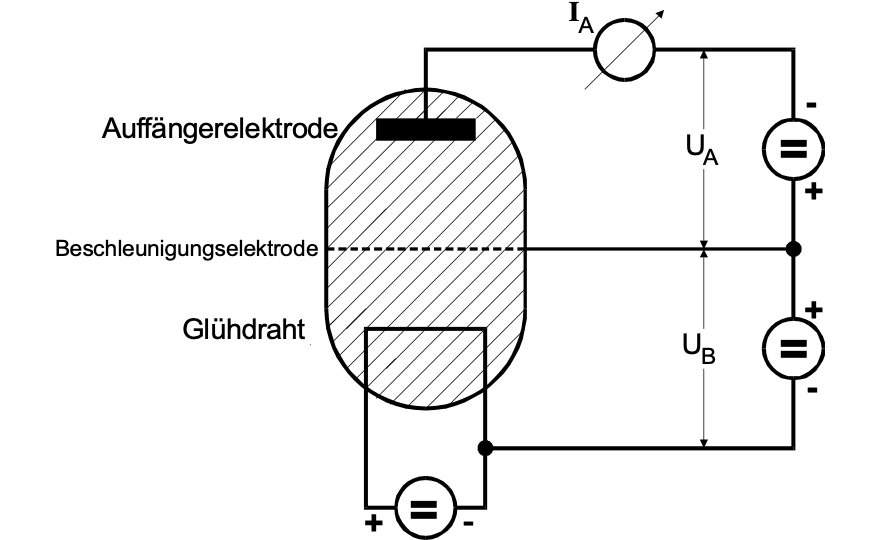
\includegraphics[width=0.6\textwidth]{content/Bilder/schematischerAufbau.png}
  \caption{Schematischer Aufbau des Franck-Hertz-Experiemtns Q\cite{anleitungV601}.}
  \label{fig:schematischerAufbau}
\end{figure}
Um die Anregungsenegie von Quecksilber zu bestimmen wird eine Franck-Hertz-Röhre verwendet, dessen schematischer Aufbau in der Abbildung \ref{fig:schematischerAufbau}
abgebildet ist. Hier befindet sich Quecksilber-Dampf in einem Glaskolben. Zusätzlich ist in dem Glaskolben ein Glühdraht, aus der durch den glühelektrischen Effekt eine 
Elektronenwolke ensteht. Diese Elektronen werden durch eine Beschleunigerspannung $U_{\text{B}}$ in Richtung der Beschleunigugnsanode hin beschleunigt. Hinter der Beschleunigugnsanode
befindet sich eine Auffängerelektrode, auf der die Elektronen landen. Während der Beschleunigugnsstrecke finden die Stoßprozesse zwischen den Elektronen und den Hg-Atomen statt. 
Die Energie der Elektronen nach den Stößen wird anhand der Gegenfeldmethode bestimmt. Die Auffängerelektrode bestizt eine geringe Gegen- bzw. Bremsspannung $U_{\text{A}}$ im Vergleich zur Beschleunigugnsanode.
Dadurch entsteht ein Bremsfeld, wogegen nur Elektronen durchgelangen für welche die kinetische Energie
\begin{equation}
  \frac{m_0}{2} v_z^2 \geq e_0 U_{\text{A}}
  \label{eqn:kinetischeEnergieUngleichung}
\end{equation}
erfüllt. Die Elektronen, die diese Ungleichung nicht erfüllen, kehren zur Beschleunigugnsanode zurück. Wird die Beschleunigerspannung kontinuierlich erhöht bis die Elektronenergie
größer oder gleich der Energie $E_{\text{a}}$ ist, werden die Hg-Atome angeregt. Dadurch besitzen die Elektronen wieder eine zu kleine Energie um gegen das Bremsfeld anzukommen.
Demnach können die Elektronen erneut Energie aufnehmen, wodurch der Verlauf des Auffängerstroms $I_{\text{A}}$ an der Auffängerelektrode im Idealfall die Franck-Hertz-Kurve
in Abbildung \ref{fig:idealeKure} abbildet.
\begin{figure}[h]
  \centering
  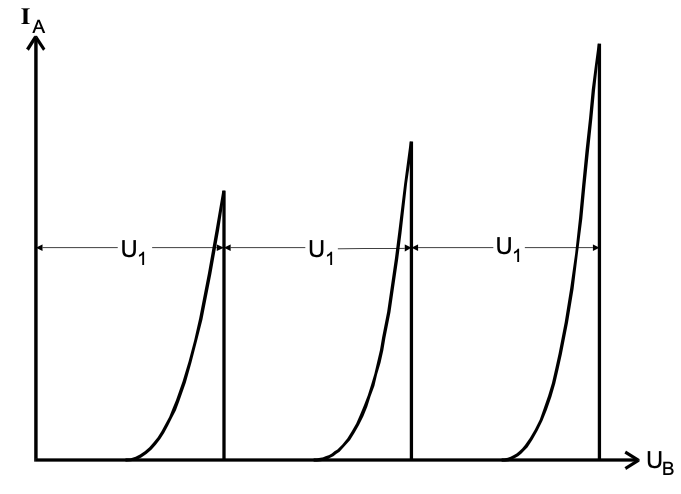
\includegraphics[width=0.6\textwidth]{content/Bilder/Ideale_Kurve.png}
  \caption{Idealisierte Franck-Hertz-Kurve Q\cite{anleitungV601}.}
  \label{fig:idealeKure}
\end{figure}
\subsection{Störquellen des Franck-Hertz-Versuchs}
\label{sec:Störquellen}
Die Kurve aus der Abbildung \ref{fig:idealeKure} lässt sich im Experiment allerdings nicht realisieren, da Nebeneffekte berücksichtigt werden müssen. Diese werden im Folgenden
weiter erläutert.
\subsubsection{Kontaktpotential}
Bei der verwendeten Franck-Hertz-Röhre bestehen die Glüh- und Beschleunigerelektrode aus unterschiedlichen Materialien, damit bei bereits relativ niedrigen Temperaturen
eine hohe Emissionsrate erzielt werden kann. Dadurch unterscheidet sich das Beschleunigungspotential von der angelegten Beschleunigungsspannung. Demnach lautet die Effektivspannung
\begin{equation}
  U_{\text{B,eff}} = U_{\text{B}} - \underbrace{\frac{1}{e_0}\left(\Phi _{\text{B}}-\Phi_{\text{G}}\right)}_{K}\,,
  \label{eqn:Effektivspannung}
\end{equation}
wobei $K$ das Kontaktpotential und $\Phi_{\text{B}}$ sowie $\Phi_{\text{G}}$ die Auftrittsarbeit der Beschleunigugnsanode und des Glühdrahts ist.
\subsubsection{Energie-Spektrum der Elektronen}
Die Elektronen besitzen beim Austreten der Glühkathode nicht dieselbe Energie, da diese bereits in der Glühkathode ein Energie-Spektrum besitzen. Dadurch fällt der
Auffängerstrom $I_{\text{A}}$ nicht bei einer genau definierten Beschleunigerspannung ab, sondern die Frank-Hertz-Kurve ist an den Peaks breiter und abgeflachter.
\subsubsection{Dampfdruck}
Damit viele Stöße zwischen den Elektronen und den Hg-Atomen zu beobachten sind, muss die mittlere freie Weglänge $\overline{w}$ der Atome klein gegenüber dem Abstand
zwischen der Glühkathode und der Beschleunigugnsanode sein. Diese Weglänge lässt sich über den Sättigungsdampfdruck 
\begin{equation}
  p_{\text{sät}} = 5,5 \cdot 10^7 \cdot \exp \left(-\frac{6876}{T}\right)
  \label{eqn:Sättigungsdampfdruck}
\end{equation}
regulieren. Hier beschreibt $T$ die Temperaturen in \unit{\kelvin} und $p_{\text{sät}}$ ist in \unit{\milli\bar}. Aus der kinetischen Gastheorie, folgt
\begin{equation}
  \overline{w} = \frac{0,0029}{p_{\text{sät}}}\,,
  \label{eqn:mittlereWeglängeAtome}
\end{equation}
mit $[\overline{w}]=\unit{\centi\metre}$. Somit exitiert ein Dampfdruckbereich, für die der Franck-Hertz-Effekt optimal verläuft. Ist die Temperatur sehr hoch,
dann treten viele elastische Stöße auf, woduch das Hg-Atom nicht angeregt wird. Bei neidrigen Temperaturen ist die Stoßwahrscheinlichkeit zu klein, sodass ebenfalls keine 
Hg-Atome angeregt werden.
